%\documentclass[11pt,fleqn]{book}%
%\documentclass{exam}%
\documentclass[11pt,a4paper]{report}
\date{{\LARGE Anno accademico 2018/2019}}
\usepackage[italian]{babel}
\usepackage[T1]{fontenc}
\usepackage{graphicx}
\usepackage[11pt]{moresize}

\font\myfont=cmr12 at 40pt
\title{{\myfont Appunti di Fisica III}}

\author{{\Huge Francesco Sacco}\\ \\ \\
		
\includegraphics[scale=0.8]{Immagini/cherubino.eps}\\}
\usepackage[utf8x]{inputenc}
\usepackage{amsmath}
\usepackage{amsthm}
\usepackage{hyperref}
\usepackage{amssymb}

\newcommand{\vettore}[1]{\mathbf{#1}}
\newcommand{\vettorec}[1]{\textrm{#1}}
\newcommand{\pscal}[2]{\langle #1,#2\rangle}
\newcommand{\pvet}[2]{#1\wedge #2}

\begin{document}
\maketitle
\tableofcontents
\newpage
\chapter{Sezione d'urto}
	Visto che c'è molta confusione sulla sezione d'urto faccio questi brevi appunti per chiarire bene cos'è e cosa rappresenta.\newline
	Lungo il pdf mettero un bel pò di note a piè di pagina, esse vanno lette solo se non si capisce quello che si sta leggendo, se stai capendo non leggerle,\footnote{Minchia ma allora non hai capito un cazzo} rovinano il flusso della discussione.\newline 
	La sezione d'urto viene indicata di solito con $\sigma$, Il suo nome richiama alla mente qualcosa che abbia a che vedere un'area su cui sbatte qualcosa. Però la sezione d'urto non è sempre l'area dell'oggetto, ma intende rappresentare una sorta di "area equivalente".\newline
	Ad esempio è ragionevole dire che per la luce l'area effettiva di un vetro $1m\times 1m$ è minore di un metro quadro, questo perchè molti fotoni passano attraverso il vetro indisturbati.\newline
	\section{Sezione d'urto s'un oggetto opaco}
	\label{sec:opaco}
		Per semplicità iniziano a trattare il concetto di sezione d'urto nel caso di un oggetto opaco,\footnote{Chiaramente le particelle incidenti sono fotoni, ma con un pò di fantasia si può generalizzare il concetto con oggetti incidenti diversi dai fotoni} in questo caso ci aspettiamo che la sezione d'urto sia uguale alla superfice ortogonale al fascio.\newline
		Noi in questo caso vogliamo ricavare l'area ortogonale in base a quello che succede al fascio di luce che lo colpisce.\newline

		Supponiamo di mandare un facio di luce con un'area maggiore del bersaglio, e che dietro ci sia uno schermo ortogonale al facio molto grande che raccolga la luce (figura \ref{fig:ombra}), allora possiamo dire che la sezione d'urto è l'area dell'ombra che l'oggetto genera sullo schermo.\newline
		Chiamarente se l'oggetto è una superfice orientata ortogonalmente al facio luminoso, la sua sezione d'urto sarà uguale alla sua area.\newline
		\begin{figure}
			\centering
    		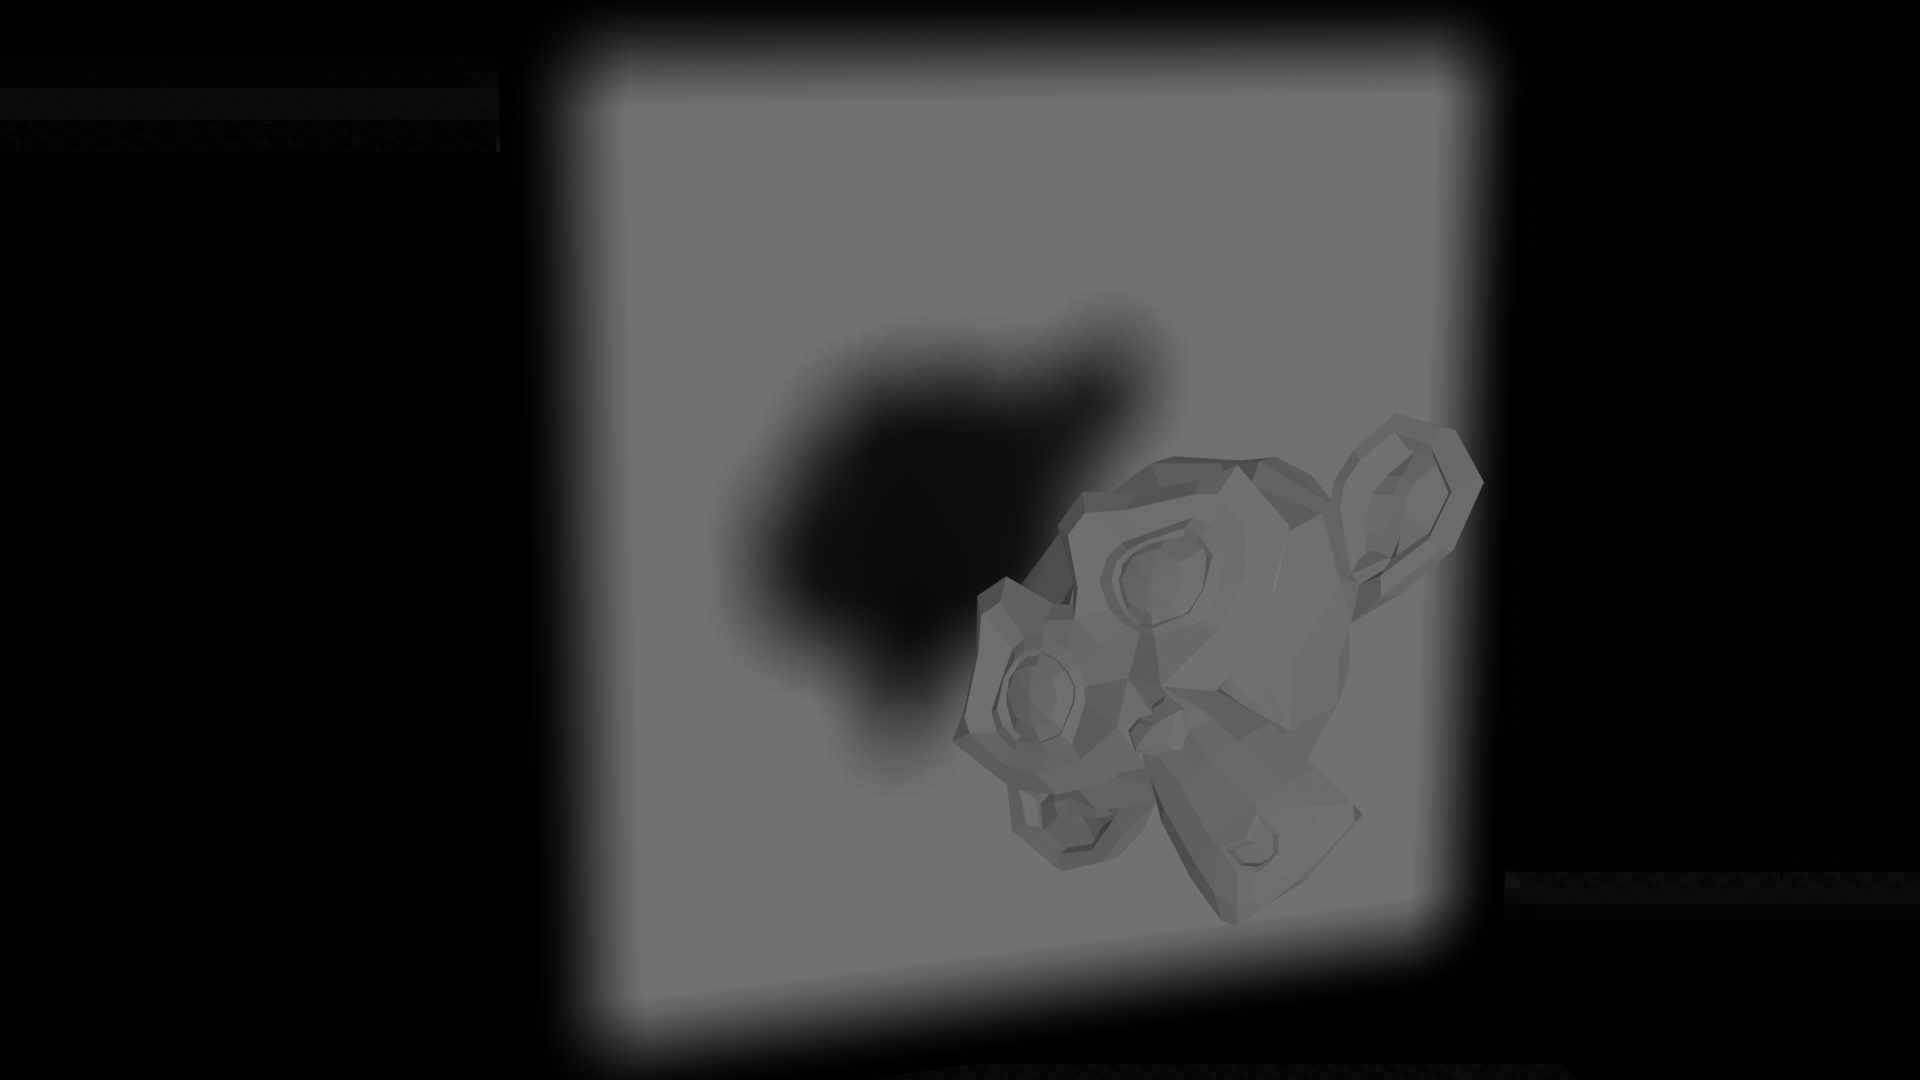
\includegraphics[width=\linewidth]{Immagini/ombra_con_blender.png}
    		\caption{Immagine fatta male illustrativa}
    		\label{fig:ombra}
		\end{figure}

		Solo che c'è un problema: nel caso di un'oggetto sgummato sarà difficile misurare l'area. Per ovviare a questo problema si può mettere uno schermo che sia in grado di contare i fotoni che riceve e una sorgente che sia in grado di contare i fotoni che manda.\newline
		Chiamiamo $A$ l'area illuminata dalla sorgente quando non c'è il bersaglio in mezzo ai piedi, che per comodità la creiamo quadrangolare, $n_s$ il numero di fotoni che colpiscono lo schermo per unità di tempo e $\Phi$ il numero di fotoni che vengono sparati dalla luce per unità di tempo, allora con una semplice proporzione si può dire che:
		\begin{equation}
			\sigma:(n_l-n_s)=A:n_l \rightarrow \sigma=A\cdot(1-n_s/\Phi)
			\label{eq:sigma_luce}
		\end{equation}
		Adesso vediamo se funziona veramente questo ragionamento.\newline
		Per verificare prendiamo un bersaglio quadrato di area $\sigma=1$ illuminata da una luce quadrata di area $A=2$, di conseguenza metà dei fotoni verrà bloccata, cioè $n_s=\Phi/2$, quindi $1=2\cdot(1-\Phi/2\cdot 1/\Phi)=2\cdot(1-1/2)=2\cdot 1/2=1$.\newline
		Che bello funziona.\newline

		Una cosa molto importante che poi verrà applicata è l'additività della sezione d'urto, infatti se prendiamo due schermi opachi quadrati con $\sigma=1$ e li mettiamo uno accanto all'altro formando un rettangolo, esso avrà una sezione d'urto uguale a $2$.

	\section{Sezione d'urto s'un oggetto traslucido}
		Per gli oggetti traslucidi tratteremo soltanto quelli planari, perchè quelli con geometri tridimenzionali si comportano in modo strano con la luce.\footnote{Facendo qualche assunzione volendo si potrebbe trattare anche oggetti tridimenzionali, ma non credo aiuti alla comprenzione del testo}\newline

		Se ti dico:"Io ho una lastra di vetro di un metro quadro che fa passare la metà della luce, qual'è la sezione d'urto?"\footnote{Supponiamo che la luce che non passi venga assorbita, a dire il vero non è molto importante che fine faccia} tu mi risponderai di sicuro:"mezzo metro quadro", ma come è possibile giustificare questa affermazione?\newline

		Chiaramente deriva dall'equazione \ref{eq:sigma_luce}, ma si perde un pò il concetto che invece era ben chiaro con lo schermo opaco che ci ha portato in primo luogo a ricavare quell'equazione.\newline

		Ora però ti porto un'altro vetro traslucido con le esatte stesse proprietà, e ti chiedo:"qual'è la sezione d'urto di quest'altro vetro?", tu mi dirai:"è lo stesso di prima, quindi per forza sarà mezzo metro quadro", e io ti rispondo:"la tua sezione d'urto è esatta, ma ti sbagli a dire che è lo stesso di prima! Questo è uno schermo opaco che ha tantissimi buchetti microscopici che in totale gli levano metà dell'area"\footnote{Chiaramente è un'esperimento mentale, nella realtà fare una cosa del genere non sarà possibile perchè dovrebbe avere uno spessore nullo e la luce ha anche un comportamento ondulatorio che porterebbe alla diffrazione, ma possiamo supporre che tutto questo non accada in questo esempio}.\newline

		Quindi effettivamente possiamo dire che il vetro è un pò come uno schermo opaco con tanti buchettini, e quindi deve avere la stessa sezione d'urto, e quindi si usa l'equazione \ref{eq:sigma_luce}.\newline

	\section{Collegamento con la probabilità}
		Sempre rimandendo nel caso del vetro traslucido posso fare questa affermazione:Se il fotone viene assorbito, allora vuol dire che ha interagito con un'atomo dell vetro, altrimenti è passato indisturbato.\newline

		Ora vogliamo vedere se è possible legare la probalbilirà di interazione $P$ con la sezione d'urto.\newline
		Sempre usando la notazione della sezione \ref{sec:opaco} e dell'equazione \ref{eq:sigma_luce}, possiamo dire che la probabilità $P$ che il fotone incida sia quanti ne vengono assorbiti dal bersaglio per unità di tempo, che sono tanti quanti a quellli che non arrivano sullo schermo per unità di tempo $N_i=(\Phi-n_s)$, diviso quanto ne arrivano in totale $\Phi$, quindi:
		\begin{equation}
			P=\frac {N_i} \Phi=\Big(1-\frac {n_s}\Phi\Big)=\frac\sigma A
			\label{eq:prob1}
		\end{equation}

	\section{Sezione d'urto di una particella}
		Supponiamo adesso che la luce venga proiettata in modo che ogni singolo fotone colpisca il bersaglio (ma non per forza deve essere assorbito, può anche attraversarlo se è translucito), e che il bersaglio sia un oggetto planare con una densità di atomi per unità di superfice $n_s$.\newline
		Adesso io voglio sapere quantè la sezione d'urto di un atomo sulla superfice, visto che la sezione d'urto è additiva\footnote{come spiegato negli ultimi righi del paragrafo \ref{sec:opaco}} posso dire che la sezione d'urto del bersagio $\sigma_b$ è uguale alla sezione d'urto di un singolo atomo $\sigma$ moltiplicato per quanti ce ne sono per unità di superfice $n_s$ moltiplicato per quanta superfice c'è $A$, quindi:
		\[
			\frac{AN_i}\Phi=\sigma_b=\sigma A n_s
		\]
		dove la prima eguaglianza viene dall'equazione \ref{eq:prob1}, risolvendo per sigma si ottiene che 
		\begin{equation}
			\sigma=\frac{N_i}{\Phi n_s}
			\label{eq:sez_lastra}
		\end{equation}
		Questa equazione però dipende da come è fatta la lastra bersaglio, quindi se vogliamo qualcosa che ne sia indipendente bisogna fare qualche passaggio matematico:
		\[
			\sigma=\frac{N_i}{\Phi n_s}\cdot \frac{An_s}{An_s}=
			\frac{N_i}{An_s}\cdot\frac A\Phi\cdot \frac {n_s}{n_s}=
			N_a\cdot \frac1{|j|}\cdot 1=\frac{N_a}{|j|}
		\]
		Dove ho detto che il numero di interazioni sulla lastra per unità di tempo $N_i$ è uguale al numero di interazioni su un singolo atomo $N_a$ moltiplicato per quanti atomi ci sono $An_s$ (Area per densità), quindi $N_i/(An_s)=N_a$ e poi ho detto che il flusso attraverso l'area $\Phi$ diviso l'area stessa $A$ dà la densità di corrente, quindi $A/\Phi=1/|j|$.\newline
		Mettendo tutti insieme si ha che 
		\begin{equation}
			\sigma=\frac{N_a}{|j|}
		\end{equation}
		Nel sistema MKS la sezione d'urto si misura in $m^2$, ma siccome essa nel caso degli atomi è circa $10^{-28}\textrm m^2$ si introduce come nuova unità di misura il barn denominata col simbolo $b$ che è uguale a $1b=10^{-28}\textrm m^2$.\newline
		Dalla relazione $h^2c^2/\textrm {GeV}^2=0.3894\textrm b$ si può usare con le unità naturali ($c=1$, $h=1$) i $\textrm {GeV}$ per misurare la sezione d'urto, in particolare $1\textrm{GeV}^{-2}=0.3894\textrm b$ oppure $1\textrm b=2.568\textrm{GeV}^{-2}$

	\section{Sezione d'urto con due gas/plasmi che si scontrano}
		\label{sec:gas}
		Fin'ora abbiamo considerato dei bersagli fermi che vengono colpiti da particelle (nello specifico fotoni), adesso considereremo ammassi di particelle che si scontrano tra di loro.\newline
		Questo è quello che succede ad esempio al CERN, dove per investigare cosa succede quando si scontrano delle particelle le une contro le altre si creano due fasci di particelle che circolano in direzione opposta ad altissima velocità e poi si mette un rilevatore nel mezzo che misura cosa avviene.\newline

		Supponiamo di avere due specie di particelle con densità per unità di volume $n_1$ e $n_2$, una velocità relativa\footnote{Si suppone per semplicità che tutte le partivelle della stessa specie viaggiano con la stessa identica velocità} $v_r$ e che ci sia un numero di interazioni per unità di volume e per unità di tempo $N$.\newline
		Adesso cerchiamo di vedere come queste variabili sono collegate con la definizione di sezione d'urto \ref{eq:sez_lastra}.\newline

		Adesso mettiamoci nel sistema di riferimento nella quale la specie 2 è ferma\footnote{Volendo potevamo prendere la specie la specie 1, tanto non cambia niente, basta che almeno una delle due stia ferma}, in questo modo la specie 2 diventa il bersaglio.\newline
		Per passare dalla densità per unità di volume $n_2$ a quella per unità di superfice $n_s$ basta moltiplicarla per $dx$ ($n_s=n_2dx$)\footnote{Questo perchè se hai in generale una funzione $f$ di cui sai $df/dV$, allora $df/dV\cdot dx=df/ds$}.\newline
		Visto che ora le particelle che si muovono sono quelli della specie 1 possiamo determinare $\Phi$, cioè il flusso di queste particelle. Visto che sappiamo la densità di volume $n_1$ delle paricelle della specie 1 e la loro velocità $v_r$, possiamo dire che $\Phi dx=n_1v_r$. Adesso mettiamo tutto in mezzo\newline
		\[
			\frac{d\sigma}{dx}=\frac{N_s}{\Phi n_s}\cdot\frac{dx}{dx}=\frac{N_s}{\Phi dx}\cdot\frac{dx}{n_s}=\frac{N_s}{n_1n_2v_r}
		\]
		dove $N_s$ sono il numero di interazioni nella superficie.\newline
		Così  peròotteniamo la sezione d'urto di un elemento di superfice con spessore infinitesimo $dx$ di gas ($d\sigma/dx$), noi vogliamo levare quel $dx$, quindi possiamo dire che il numero di interazioni per unità di superfice, integrato in dx darà il numero di interazioni in tutto il volume, cioè $\int N_sdx=N_v$, quindi.
		\begin{equation}
			\sigma=\frac{N_v}{n_1n_2v_r}
			\label{eq:gas}
		\end{equation} 


	\section{Sezione d'urto differenziale e Scattering Rutherford}
		Alcune sezioni d'urto per loro natura tendono a divergere. Infatti se consideriamo lo scattering Coulomb tra un flusso di particelle cariche $|j|$ che incide su una carica dello stesso segno si ha che $\sigma=N/|j|=+\infty$ visto che il numero di interazioni al secondo è infinito se consideriamo il flusso incidente come un'infinità di particelle che arrivano al secondo.\newline
		Questo torna al livello intuitivo perchè se la sezione d'urto è l'area all'interno del quale c'è interazione tra proiettile e bersaglio, allora nel caso dell'interazione eletromagnetica deve fare infinito visto che il campo elettrico di una carica si estende all'infinito.\footnote{Ciò che conta nella sezione d'urto è se un'interazione c'è o no, quindi anche una particella che passa molto lontana dal bersagio è considerata come se interaggisse con esso nonostante il fatto che il campo elettrico è debole e quindi viene deflessa minimamente}\newline
		Però abbiamo detto che sezione d'urto e probabilità vanno a braccetto, quindi certe volte anzichè chiedersi "Qual'è la probabilità che ...", si ci può chiedere "Qual'è la sezione d'urto tale che ...". Nei puntini chiaramente si ci deve mettere qualcosa che abbia senso nel nostro contesto.\newline

		Adesso ci chiediamo qual'è la sezione d'urto tale che il flusso uscente finisca per andare entro un certo angolo solido infinitesimo $d\Omega$ dopo che avvenga uno scattering coulumbiano. Scritto in equazioni sarà così:
		\begin{equation}
			\frac{d\sigma}{d\Omega}=\frac{N(\Omega)}{|j|}
			\label{eq:sez_diff}
		\end{equation}
		$d\sigma$ rappresenta una piccola area, tale che se ci entri poi vai a finire in un angolo solido $d\Omega$, (immagine \ref{fig:rut1}) e $N(\Omega)$ è il numero di interazioni al secondo che fanno finire asintoticamente i proiettili in un angolo $\Omega$.\newline
		\begin{figure}
			\centering
    		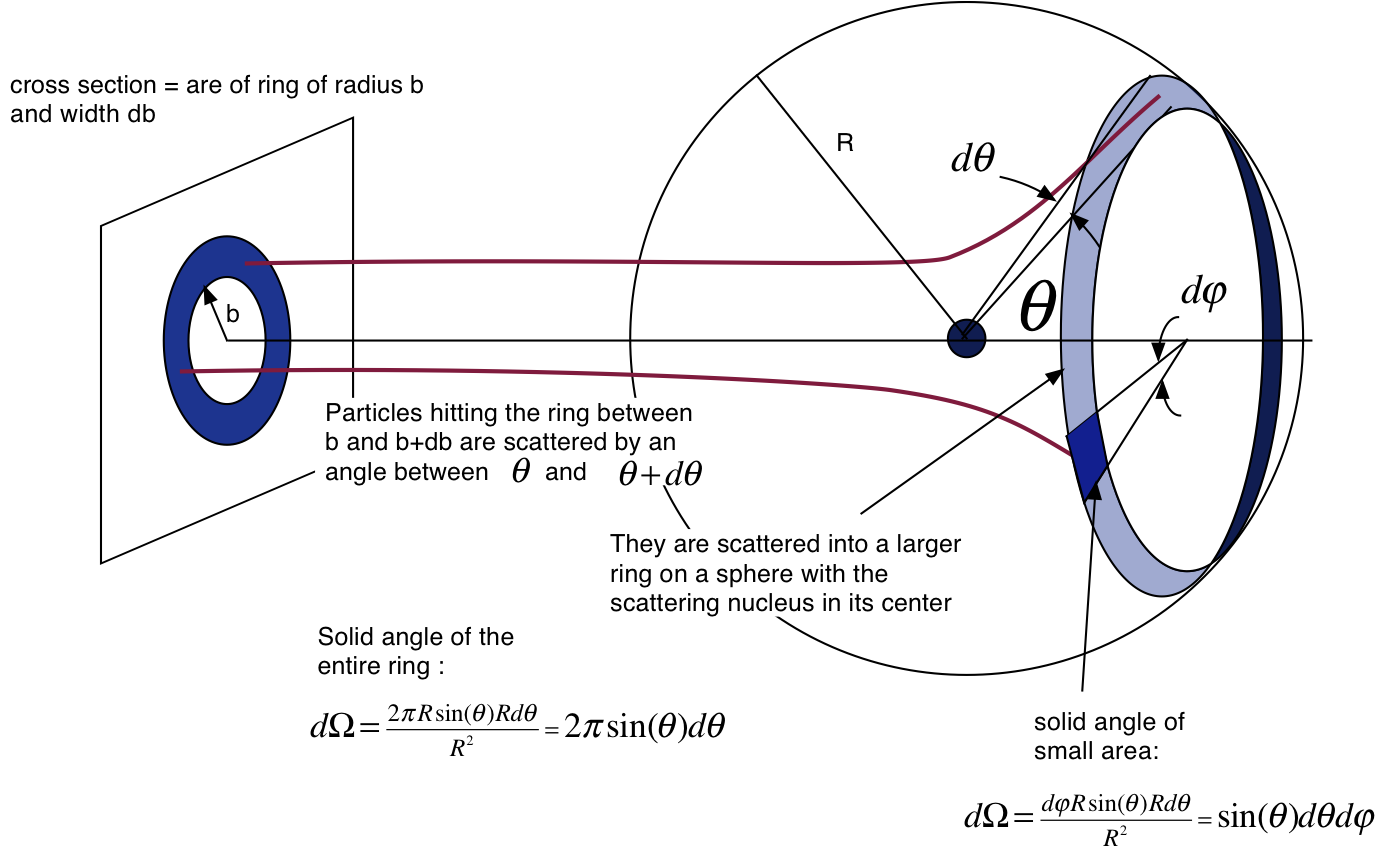
\includegraphics[width=\linewidth]{Immagini/solid_angle.png}
    		\caption{In questo caso $d\sigma=2\pi b db$ e $d\Omega=2\pi \sin(\theta)d\theta$ sono a simmetria cilindrica}
    		\label{fig:rut1}
		\end{figure}
		Questo tipo di scattering è detto "Scattering Rutherford", non mi dedicherò molto a questo argomento perchè è trattato abbastanza bene anche altrove\footnote{Ad esempio nelle dispenze di Claudio Bonati}. Qui dirò soltanto che il risultato finale è che
		\begin{equation}
			\frac{d\sigma}{d\Omega}=\Big(\frac{e_1e_2}{2\mu v_\infty^2 }\Big)^2\frac{1}{\sin^4(\theta/2)}
		\end{equation}
		dove $\mu$, $e_2$, $v_\infty$ e $\theta$ sono rispettivamente la massa, la carica, la velocità iniziale e l'angolo di deflessione delle particelle cariche proiettile ed $e_1$ è la carica del bersaglio.\newline
		La correzzione dello scattering Rutherford che tiene contro dello spin dell'elettrone incidente sul nucleo e degli effetti relativistici è detto scattering Mott ed è uguale a\footnote{Per spiegare il perchè di questa equazione serve la teoria quantistica dei campi, quindi a meno che tu non abbia le basi per capirla di consiglio di prenderla per buona}
		\begin{equation}
			\frac{d\sigma}{d\Omega}\Big|_{Mott}=\frac{d\sigma}{d\Omega}\Big|_{Ruth}\Big(1-\beta ^2\sin ^2\frac\theta 2\Big)
		\end{equation}
		Lo scattering Rutherford può essere usato per determinare la dimenzione del nucleo.\newline
		Nel caso di scattering di particelle $\alpha$\footnote{Nuclei di He$_4$, cioè formati da 2 protoni e due neutroni} si osserva sperimentalmente che le previsioni teoriche sono corrette per energie cinetiche  $\lesssim 30$MeV. Quindi eguagliando l'energia potenziale a $30$MeV otteniamo una stima approssimativa del raggio atomico, quindi $30 \textrm{MeV}\lesssim E=e^2z_\alpha z_A/R$. Risolvendo per il raggio atomico $R$ si ottiene
		\begin{equation}
			R\lesssim\frac{e^2z_A}{15 \textrm{MeV}}
		\end{equation}
		Dove $z_A$ è il numero atomico dell'atomo colpito e ho diviso per due perchè il numero atomico della particella $\alpha$ ($z_\alpha$) è sempre uguale a $2$


	\section{Cose con onde elettromagnetiche}
		Nel caso di onde elettromagnetiche si ci può chiedere:"Una volta che ci siamo calcolati come delle onde elettromangetiche di frequenza $\omega$ vengono diffratte da un'ostacolo, non possiamo calcolarci la sezione d'urto come se fosse stata calcolata con dei fotoni anch'essi di frequenza $\omega$?".\newline
		Effettivamente, se fosse possibile farlo risolverebbe un bel pò di problemi: prima di tutto la necessità di considerare come proiettili delle cose che in un modo o nell'altro sono discrete, ma fare il tutto con dei campi.\newline
		Immagginato di esser stati bravi ad aver calcolato i campi del problema che stiamo analizzato, cioè
		\[
			\begin{cases}
				E=E_{i}+E_{s}\\
				B=B_{i}+B_{s}

			\end{cases}
		\]
		\begin{figure}
			\centering
    		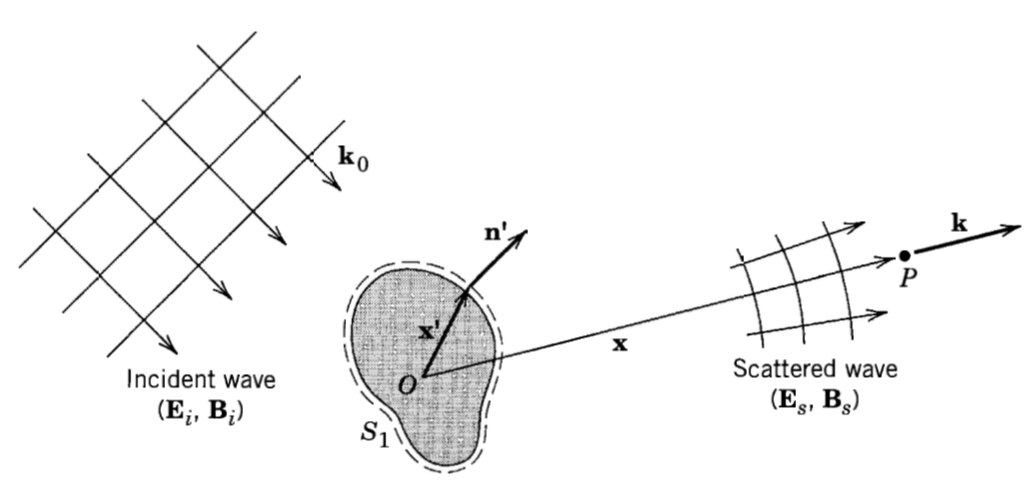
\includegraphics[width=\linewidth]{Immagini/irraggiamento.png}
    		\caption{Onda incidente e onda rifratta}
    		\label{fig:irr}
		\end{figure}
		Dove $E_{i}$ e $E_{s}$ indicano i campi elettrici incidenti e irraggiati (figura \ref{fig:irr}),\footnote{è scirtto $E_s$ perchè la $s$ sta per scattered (irraggiato in inglese)} stessa cosa vale per il campo magnetico.\newline
		Visto che $\pscal{\langle\vettore S \rangle}{d\vettore{a}}$ è uguale al flusso di potenza, che è uguale a quanti fotoni passano attraverso $d\vettore a$ per unità di tempo moltiplicato per quanta energia ha ognuno di loro. Scritto in matematichese $\hbar \omega \phi$=$\hbar \omega \pscal{\vettore j}{d\vettore a}$, quindi
		\begin{equation}
			\pscal{\langle\vettore S \rangle}{d\vettore{a}}=\hbar \omega \pscal{\vettore j}{d\vettore a}
			\rightarrow
			\langle\vettore S\rangle= \hbar \omega\vettore j
		\end{equation}
		dove $\vettore S=\frac{1}{\mu_0}\pvet{\Re(\vettore E)}{\Re(\vettore B)}$, e $\vettore j$ è lo stesso che va a finire nel denominatore dell'equazione \ref{eq:sez_diff}.\newline
		Ricordiamo la definizione della sezione d'urto differenziale: $\frac{d\sigma}{d\Omega}=N(\Omega)/|j|$ (eq \ref{eq:sez_diff}).
		\[
			d\sigma=\frac{N(\Omega)d\Omega}{|j|}\cdot\frac{\hbar\omega}{\hbar \omega}=
			\frac{\hbar \omega N(\Omega)d\Omega}{|\langle \vettore S_i\rangle|}
		\]
		Adesso concentriamoci col significato di $\hbar \omega N(\Omega)d\Omega$, esso è uguale a quanti fotoni vanno nella direzione dell'angolo infinitesimo $d\Omega$ moltiplicato per la loro energia.\newline
		Quindi possiamo dire che se lo moltiplichiamo per la superfice che essi attraversano ($R^2d\Omega $) otteniamo potenza irraggiata nell'angolo $d\Omega$.\newline
		Esso è uguale al flusso del vettore di poyinting attraverso la stessa superfice, che è $R^2|\langle \vettore {S}_s \rangle |d\Omega $. Quindi mettendo tutto dentro si ha che
		\[
			d\sigma=\frac{\hbar \omega N(\Omega)d\Omega}{|\langle \vettore S_i\rangle|}=
			\frac{R^2|\langle \vettore S_s(\Omega) \rangle |d\Omega}{|\langle \vettore S_i\rangle|}
		\]
		adesso basta riportare il differenziale a sinistra e si ottiene la formula della sezione d'urto differenziale
		\begin{equation}
			\frac{d\sigma}{d\Omega}=\frac{R^2|\langle \vettore S_s(\Omega) \rangle |}{|\langle \vettore S_i\rangle|}
		\end{equation}

	\section{Cose con lo spazio delle fasi}
		Due sezioni fà (sez.\ref{sec:gas}) abbiamo calcolato la sezione d'urto differenziale per una deflessione in un generico angolo $\Omega$.\newline
		Possiamo generalizzare il concetto di sezione d'urto differenziale nel caso di un numero arbitrario di parametri finali di un'esperimento di scattering.\footnote{Si possono tenere in considerazione anche i parametri iniziali, ma per ora li ignoriamo}\newline
		Supponiamo di avere una reazione del tipo:
		\begin{equation}
			a+b\rightarrow c_1+c_2+\dots+c_n
		\end{equation}
		Che equivale a dire di supporre che siamo nella situazione che due particelle si scontrano e producono $n$ particelle.\newline
		Per rendere meglio l'idea supponiamo che l'esperimento per la misura della sezione d'urto di questo esperimento sia fatto da due gas o plasmi che si muovono in direzione opposta come nella sezione \ref{sec:gas}.\footnote{Questo non è del tutto necessario, ma serve a darci l'idea, in ogni caso alla fine del paragrafo generalizzeremo}\newline
		Supponiamo di avere un rivelatore molto buono che sia in grado di rilevare il quadrimpulso di ogni singola particella uscente dal processo.\newline

		Siano $\vettore P_1,\dots, \vettore P_n$ i quadrimpulsi delle particelle $c_1,\dots,c_n$, sia \\$N_v(\vettore P_1,\dots,\vettore P_n)d\vettore P_1\dots d\vettore P_n$ il numero di eventi per unità di volume, per unità di tempo che abbiano una reazione che facciano finire la reazione nell'insieme dello spazio delle fasi $\vettore P_1+d\vettore P_1,\dots,\vettore P_n +d\vettore P_n $,\footnote{Cioè un cubetto con uno spigolo in $(\vettore P_1,\dots,\vettore P_n)$ e l'altro in $\vettore P_1+d\vettore P_1,\dots,\vettore P_n +d\vettore P_n $ e tutti i lati paralleli agli assi cartesiani}.\newline
		Dall'equazione \ref{eq:gas} discende che 
		\begin{equation}
			d\sigma=\frac{N_v(\vettore P_1,\dots,\vettore P_n)}{n_1n_2v_r}d\vettore P_1\dots d\vettore P_n
		\end{equation}
		Dove le variabili al denominatore sono le stesse dell'equazione \ref{eq:gas}.\newline
		Bisogna però tenere in considerazione il fatto che i gradi di libertà non sono $4n$, ma sono di meno a causa della conservazione del quadrimpulso iniziale e dal fatto che la norma di un quadrimpulso è sempre uguale alla massa a riposo della particella moltiplicata per la velocità della luce, quindi i gradi di libertà in realtà sono $3n-1$.\newline
		Imponendo questi vincoli si ottiene un sottoinsieme dello spazio delle fasi su cui è possibile lavorare più semplicemente. Sensa perdersi troppo nella matematica ti sbatto in faccia il risultato:
		\begin{equation}
			d\vettore \Gamma=\delta^4\bigg(\vettore P_t-\sum_i^n \vettore P_i\bigg)\prod_i^n\frac{d^3\vettore p_i}{2E_i}
		\end{equation}
		dove $p_i$ è la parte spaziale di $P_i$ e $E_i$ la parte temporale.\newline
		Mettendo tutto assieme si ottiene che 
		\begin{equation}
			d\sigma=\frac{N_v(\vettore p_1,\dots,\vettore p_n)}{n_1n_2v_r}\delta^4\bigg(\vettore P_t-\sum_i^n \vettore P_i\bigg)\prod_i^n\frac{d^3\vettore p_i}{2E_i}
		\end{equation}
		Visto che non è detto che l'esperimento venga fatto con due plasmi che si scontrano non è detto che l'equazione che determina dalla sezione d'urto sia sempre come quella qua sopra, in generale il numero di eventi per unità di volume, per unità di tempo che abbiano una reazione che facciano finire la reazione in $d\vettore \Gamma$ è una generica funzione $f(\vettore p_1,\dots,\vettore p_n)$.\newline
		Quindi la sezione d'urto differenziale generica rispetto allo spazio delle fasi è
		\begin{equation}
			d\sigma=f(\vettore p_1,\dots,\vettore p_n)\delta^4\bigg(\vettore P_t-\sum_i^n \vettore P_i\bigg)\prod_i^n\frac{d^3\vettore p_i}{2E_i}
			\label{eq:spaz_fas}
		\end{equation} 
		Per qualche strana ragione questa definizione di sezione d'urto viene usata anche nei decadimenti, anche se non capisco che c'azzecca, cioè la sezione d'urto è un'area, non una probabilità, come fanno a determinare la costante di normalizzazione?\newline
		Forse si sfrutta la parametrizzazione della sezione d'urto in GeV e a quel punto si normalizza in modo che la sezione d'urto totale sia uguale all'energia rilasciata nel processo decadimento, ma non ne sono certo e comunque non vedo che senso abbia, a me sembra abbastanza arbitraria come cosa.


	\section{Processi inclusivi}
		In realtà non sempre è possibile misurare il quadrimpulso di ogni particella uscente da un urto, quindi difficilmente si può usare la definizione di sezione d'urto dell'ultima equazione scritta (eq.\ref{eq:spaz_fas}).\newline
		In fisica i processi nei quali è possibile misurare il quadrimpulso di ogni particella sono detti processi processi "esclusivi", come per esempio l'urto tra due palle di biliardo, altrimenti sono detti "inclusivi", come in molti esperimenti di fisica delle alte energie.\newline
		Ad esempio se siamo soltanto in grado di misurare l'energia della particella $i-$esima, allora l'equazione diventa così:
		\begin{equation}
			d\sigma=f(E_i)dE_i
		\end{equation}
		dove $f(E_i)$ ha lo stesso significato della $f(\vettore p_1,\dots,\vettore p_n)$ dell'ultima equazione (eq.\ref{eq:spaz_fas})


















\chapter{Elettromagnetismo}
	Qua metterò solo le cose da imparare a memoria di elettromagnetismo, se vuoi studiare l'elettromagnetismo necessario per Fisica 3 vai a leggerti le dispense di Bonati
	\section{Equazioni di Maxwell}
		Nel sistema internazionale (SI):
		\begin{equation}
			\begin{cases}
				\pscal \nabla{\vettore E}=\rho/\epsilon_0\\
				\pvet \nabla {\vettore E}=-\frac{\partial \vettore B}{\partial t}\\
				\pscal \nabla{\vettore B}=0\\
				\pvet \nabla {\vettore B}=\mu_0\vettore J+\mu_0\epsilon_0\frac{\partial \vettore E}{\partial t}
			\end{cases}
			\begin{cases}
				\pscal \nabla{\vettore D}=\rho\\
				\pvet \nabla {\vettore E}=-\frac{\partial \vettore B}{\partial t}\\
				\pscal \nabla{\vettore B}=0\\
				\pvet \nabla {\vettore H}=\vettore J+\frac{\partial \vettore D}{\partial t}
			\end{cases}
		\end{equation}
		Nel sistema Gaussiano (G):
		\begin{equation}
			\begin{cases}
				\pscal \nabla{\vettore E}=4\pi\rho\\
				\pvet \nabla {\vettore E}=-\frac 1 c \frac{\partial \vettore B}{\partial t}\\
				\pscal \nabla{\vettore B}=0\\
				\pvet \nabla {\vettore B}=\frac{4\pi}c \vettore J+\frac 1 c \frac{\partial \vettore E}{\partial t}
			\end{cases}
		\end{equation}
		Per ricordarsi del sistema gaussiano basta pensare che la forza di Coulomb è $q_1q_2/r^2$ e la forza di Lorentz è $q(\vettore E+\pvet{\vettore \beta}{\vettore B})$

	\section{Conversione SI-G}
		Per passare dal sistema internazionale a quello gaussiano basta usare queste 3 equazioni. $k_0=1/\sqrt{4\pi\epsilon_0}$
		\begin{equation}
			\begin{cases}
				(\vettore E,\phi)|_G=1/k_0(\vettore E,\phi)|_{SI}\\
				(\vettore J, \rho)|_G=k_0(\vettore J, \rho)|_{SI}\\
				(\vettore B,\vettore A)_G=c/k_0(\vettore B,\vettore A)_{SI}=
				\sqrt{\frac{4\pi}{\mu_0}}(\vettore B,\vettore A)_{SI}
			\end{cases}
		\end{equation}



	\section{Formule utili}
		\subsection{Densità di Energia}
			\begin{equation}
				W=\frac{E^2+B^2}{8\pi}\quad(\textrm{G})\quad=\quad\frac{\epsilon_0}{2}(E^2+c^2B^2)\quad(\textrm{SI})
			\end{equation}
		\subsection{Vettore di Poynting}
			\begin{equation}
				\vettore S=\frac c{4\pi}(\pvet{\vettore E}{\vettore B})\quad(\textrm{G})\quad=\quad\frac{1}{\mu_0}(\pvet{\vettore E}{\vettore B})\quad(\textrm{SI})
			\end{equation}
		\subsection{Tensore Impulso}
			Per ricordarlo meglio bisogna pensare di mettere lungo la diagonale l'energia e poi sottrarre in tutta la matrice i campi incrociati
			\begin{equation}
				\sigma_{ij}=\frac 1{4\pi}\bigg[\frac{\delta_{ij}}2(E^2+B^2)-E_iE_j-B_iB_j\bigg]\quad(\textrm {G})
			\end{equation}
			\[
				\sigma_{ij}=\epsilon_0\bigg[\frac{\delta_{ij}}2(E^2+c^2B^2)-E_iE_j-c^2B_iB_j\bigg]\quad(\textrm {SI})
			\]


		\subsection{Tensore di campo}
			\begin{equation}
				F^{\mu\nu}=\partial^\mu A^\nu-\partial^\nu A^\mu=
				\begin{vmatrix}
					0 & -\vettorec E_x & -\vettorec E_y & -\vettorec E_z\\
					\vettorec E_x & 0 & -\vettorec B_z & \vettorec B_y\\
					\vettorec E_y & \vettorec B_z & 0 & -\vettorec B_x\\
					\vettorec E_z & -\vettorec B_y & \vettorec B_x & 0
				\end{vmatrix}
			\end{equation}

			Tensore duale 
			\[
			\mathcal F^{\alpha\beta}=\frac 1 2\epsilon^{\alpha\beta\gamma\delta}F_{\gamma\delta}
			\]

			Equazioni di Maxwell:
			\begin{equation}
				\partial_\mu F^{\mu\nu}=\frac{4\pi}{c}j^\nu,\quad\quad\partial_\alpha\mathcal F^{\alpha\beta}=0
			\end{equation}

			Forza di Lorentz:
			\begin{equation}
				\frac 1 c F^{\mu\nu}j_\nu=\frac{dp^\mu}{dt}
			\end{equation}




		\subsection{Tensore Enegia-Impulso}
			\begin{equation}
				T^{\mu\nu}=
				\begin{vmatrix}
					W & \vettore S/c\\
					\vettore S/c & \sigma_{ij}
				\end{vmatrix}
			\end{equation}

		\subsection{Trasformazione dei Campi}
			\begin{equation}
				\begin{cases}
					\vettore E'_{//}=\vettore E_{//}\quad \vettore B'_{//}=\vettore B_{//}\\
					\vettore E'_{\bot}=\gamma(\vettore E_\bot+
					\pvet{\vettore\beta}{\vettore B_\bot})\\
					\vettore B'_{\bot}=\gamma(\vettore B_\bot-
					\pvet{\vettore\beta}{\vettore E_\bot})
				\end{cases}
			\end{equation}

	\section{Radiazione}
		Partiamo con un pò di notazione:
		\begin{itemize}
			\item $\vettore r$ è il punto nel quale si osservano i campi (una specie di origine)
			\item $t$ è il momento nel quale si osservano i campi
			\item $\vettore r'$ è la posizione della sorgente
			\item $t'$ è il tempo ritardato, deriva da $c(t-t')=|\vettore r-\vettore r'(t')|$
			\item $\vettore R=\vettore r-\vettore r'(t')$ è il vettore che parte da $\vettore r'$ e finisce in $\vettore r$
			\item $\hat{\vettore n}=\vettore R/\vettorec R$
			\item $\beta=\frac1c\frac{d\vettore r'}{dt}$
			\item $\gamma=\frac 1{\sqrt{1-\beta^2}}$
		\end{itemize}
		\subsection{Campi generati da una carica $q$ in un moto generico}
			Il termine a destra del campo elettrico è quello più importante da imparare a memoria esso rappresenta il campo elettrico molto lontano visto che va come $1/R$.
			\begin{equation}
				\vettore E(\vettore r,t)=\frac q{\gamma^2R^2}\frac{\hat{\vettore n}-\vettore \beta}{(1-\pscal{\hat{\vettore n}}{\vettore \beta})^3}\bigg|_{t_r}+
				\frac{q}{cR}
				\frac{\pvet{\hat{\vettore n}}{\big[\pvet{(\hat{\vettore n}-\vettore \beta)}{\dot{\vettore \beta}}\big]}}{(1-\pscal{\hat{\vettore n}}{\vettore \beta})^3}\bigg|_{t_r}\quad(\textrm {G})
				\label{eq:Eirr}
			\end{equation}
			\[
				B=\pvet{\hat{\vettore n}}{\vettore E}|_{t_{rit}}
			\]
		\subsection{Radiazione sviluppata al secondo ordine non relativistica}
			\begin{equation}
				I=\frac{2}{3c^2}(\ddot p^2+\ddot m^2)+\frac{\sum_{ij}\dddot Q_{ij}\dddot Q_{ij}}{180c^5}\quad(\textrm {G})
			\end{equation}

	\section{Attraversamento della materia di particelle cariche}
		Altra notazione:
		\begin{itemize}
			\item $\alpha=e^2/(\hbar c)\approx 1/137$ costante di struttura fine
			\item $m_e=0.51$MeV$/c^2$
			\item $r_e=e^2/(m_ec^2)\approx 2.8$fm raggio classico dell'elettrone
		\end{itemize}
		sia $\frac{d\mathcal{E}}{d\Omega}$ l'energia irraggiata per unità di angolo solido, essa è uguale a
		\begin{equation}
			\frac{d\mathcal{E}}{d\Omega}=\frac{c}{4\pi}\int_{-\infty} ^{+\infty} R^2\vettorec E^2 dt
		\end{equation}
		Il campo elettico è quello dell'equazione \ref{eq:Eirr} nel nostro caso consideriamo la forza agente sulla particella esclusivamente perpendicolare al suo moto caso, e quindi si può scrivere
		\begin{equation}
			R\vettore E=\frac{q}{c}\pvet{\hat{\vettore n}}{\big(\pvet{\hat{\vettore n}}{\dot{\vettore \beta}}\big)}
		\end{equation}
		La trasformata dell'equazione di sopra è 
		\begin{equation}
			\int_{-\infty} ^{+\infty} \frac{e^{i\omega t}}{\sqrt{2\pi}}\frac{q}{c}\pvet{\hat{\vettore n}}{\big(\pvet{\hat{\vettore n}}{\dot{\vettore \beta}}\big)} dt
		\end{equation}
		Sfruttanto che la trasformata definita così è isometrica si ha che
		\begin{equation}
			\frac{d\mathcal{E}}{d\Omega}=\int_{-\infty} ^{+\infty} 
			\frac{e^2}{8\pi^2 c}\Bigg|\int_{-\infty} ^{+\infty}e^{i\omega t}\frac{q}{c}\pvet{\hat{\vettore n}}{\big(\pvet{\hat{\vettore n}}{\dot{\vettore \beta}}\big)} dt\Bigg|^2
			d\omega=
		\end{equation}
		\[
			=\frac{e^2}{4\pi^2 c}\int_0 ^{+\infty} 
			\Bigg|\int_{-\infty} ^{+\infty}e^{i\omega t}\frac{q}{c}\pvet{\hat{\vettore n}}{\big(\pvet{\hat{\vettore n}}{\dot{\vettore \beta}}\big)} dt\Bigg|^2
			d\omega	
		\]
		Quindi si può decidere (in modo abbastanza improprio) che 
		\begin{equation}
			\frac{d^2\mathcal{E}}{d\Omega d\omega}=\frac{e^2}{4\pi^2 c}\Bigg|\int_{-\infty} ^{+\infty}e^{i\omega t}\frac{q}{c}\pvet{\hat{\vettore n}}{\big(\pvet{\hat{\vettore n}}{\dot{\vettore \beta}}\big)} dt\Bigg|^2
		\end{equation}
		$\pvet{\hat{\vettore n}}{\big(\pvet{\hat{\vettore n}}{\dot{\vettore \beta}}\big)}=\dot{\vettore \beta}\sin(\theta)$.\newline
		nel caso $\omega\tau\gg1$ allora la trasformata si annulla perhcè c'è interferenza, nel caso opposto invece la funzione rimane para para: 
		\begin{equation}
			\frac{d^2\mathcal{E}}{d\Omega d\omega}=
			\begin{cases}
				\frac1c \Big(\frac{q|\Delta \vettore v|\sin(\theta)}{2\pi c}\Big)^2\textrm{ per } \omega\tau\lesssim 1 \\
				0 \textrm{ per }\omega\tau\gtrsim 1
			\end{cases}
		\end{equation}
		Se si suppone che l'angolo di deflessione sia piccolo, allora si può dire che la variazione di velocità è pari alla forza subita nella direzione ortogonale al moto, facendo qualche conto si ottiene che 
		\[
			|\Delta \vettore v|=\frac{2qQ}{bmv}
		\]
		dove $Q$ è la massa del coso colpito e m la massa del proiettile. Dopo aver integrato in tutti gli angoli solidi e imposto che $\tau\approx b/v$ si ottiene che 
		\begin{equation}
			\frac{d\mathcal{E}}{d\omega}=
			\begin{cases}
				\frac8{3c^3\pi }\Big(\frac{q^2Q}{bmv}\Big)^2\textrm{ per } \omega\lesssim v/b \\
				0 \textrm{ per }\omega\gtrsim v/b
			\end{cases}
		\end{equation}

		Adesso voglio vedere quanta energia viene irradiata per unità di frequenza se ci faccio passare un flusso di particelle attorno al bersaglio.\newline
		\begin{equation}
			\frac{d\chi}{d\omega}=\int_{b_{min}}^{b_{max}}2\pi b  \frac{d\mathcal{E}}{d\omega}db=\frac1{3c^3 }\Big(\frac{4q^2Q}{mv}\Big)^2\int_{b_{min}}^{b_{max}} \frac{db}b
		\end{equation}

		Adesso bisogna scegliere bene $b_{max}$ e $b_{min}$.\newline
		I valori cambiano a seconda se si è nel caso relativistico o in quello non relativistico.\newline
		$b_{max}=\min\{a,v\gamma/\omega\}$, per $\gamma$ grandi si prende il raggio atomico $a$, nel caso non relativistico si sceglie $v/\omega$.\newline
		dal principio di indeterminazione si ha che $\Delta \vettore x\Delta \vettore v=\hbar/m$, se si suppone per eccesso che $\Delta \vettore v\lesssim \vettore v$ e al posto di $\vettore x $ si ci metter $b$ si ottiene che $b_{min}=\hbar/mv$.\newline
		mettendo tutto inzieme si ottiene 
		\begin{equation}
			\frac{d\chi}{d\omega}=\frac1{3c^3 }\Big(\frac{4q^2Q}{mv}\Big)^2
			\ln\bigg(\frac{mv\min\{a,v\gamma/\omega\}}{\hbar}\bigg)
		\end{equation}
		Integrando nelle frequenze da $0<\omega<E/\hbar$ e moltiplicanto per il numero di nuclei per unità di volume $n$ si ottiene che 
		\begin{equation}
			\frac{dE}{dx}=n\int_0^E/\hbar
		\end{equation}
	\end{document}